\section{Bài toán 5: Dùng Solidity xây dụng smart contract}

\subsection{Hiện thực code bằng Solidity}
Dưới đây là phần hiện thực smart contract trên bằng Solidity, có thể chạy trên môi trường remix của ethereum. Mã nguồn gồm 2 file tương ứng 2 smart contract được hiện thực. Smart contract đầu tiên là Transport hiện thực nội dung của bản hợp đồng trên. Trong smart contract này, có sử dụng một smart contract khác là DateTime, đây là một open source trên mạng lưới ethereum, hỗ trợ chuyển đổi thời gian trên hệ thống ethereum.

\vspace{1cm}
\textbf{Đây là smart contract Transport:}

\lstinputlisting[language=JavaScript]{code/Transport.js}


\vspace{1cm}
\textbf{Đây là smart contract DateTime:}

\lstinputlisting[language=JavaScript]{code/DateTime.js}


\subsection{Ảnh minh họa cho việc chạy trên môi trường remix}

\begin{figure}[tph]
	\centering
	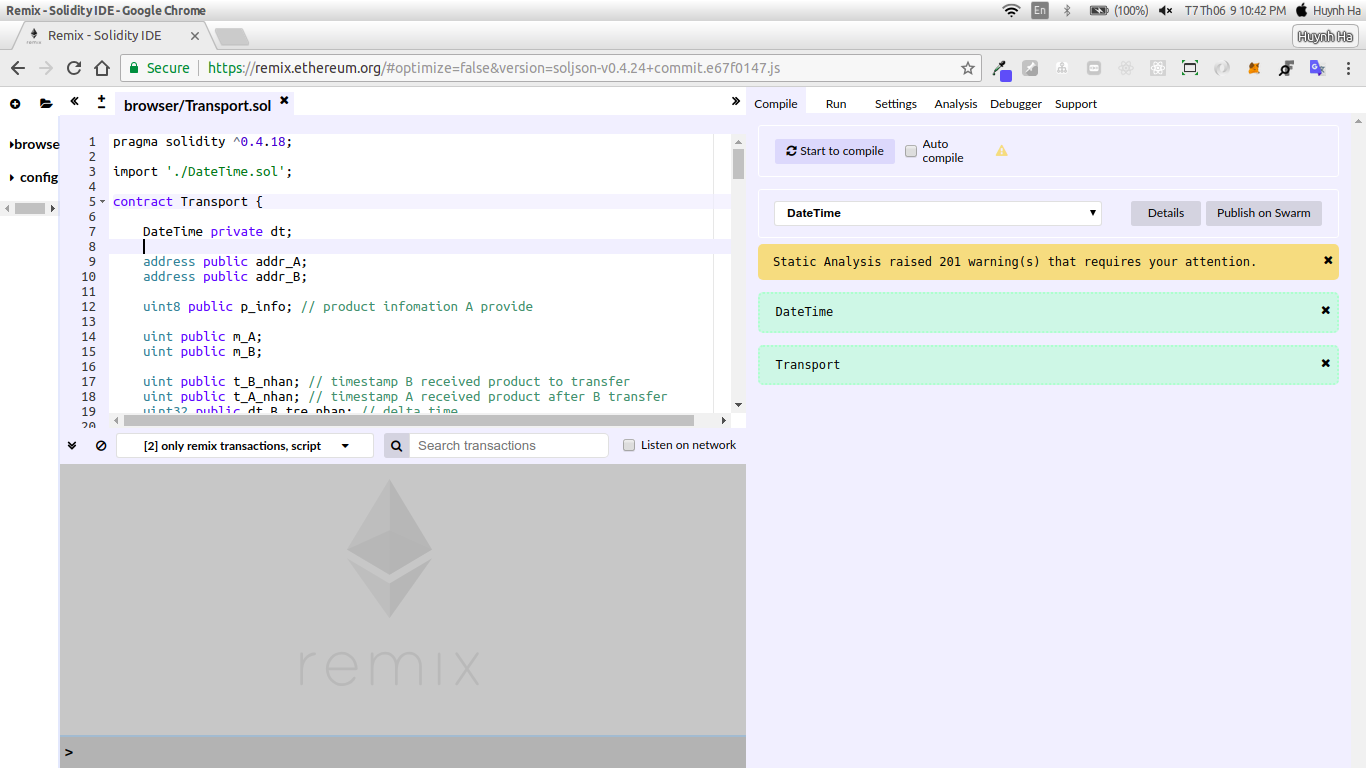
\includegraphics[width=14cm]{snapshot/1.png}
	\vspace{0.3cm}
	\caption{Compile smart contract}
	\label{fig:fig1}
\end{figure}

\begin{figure}[tph]
	\centering
	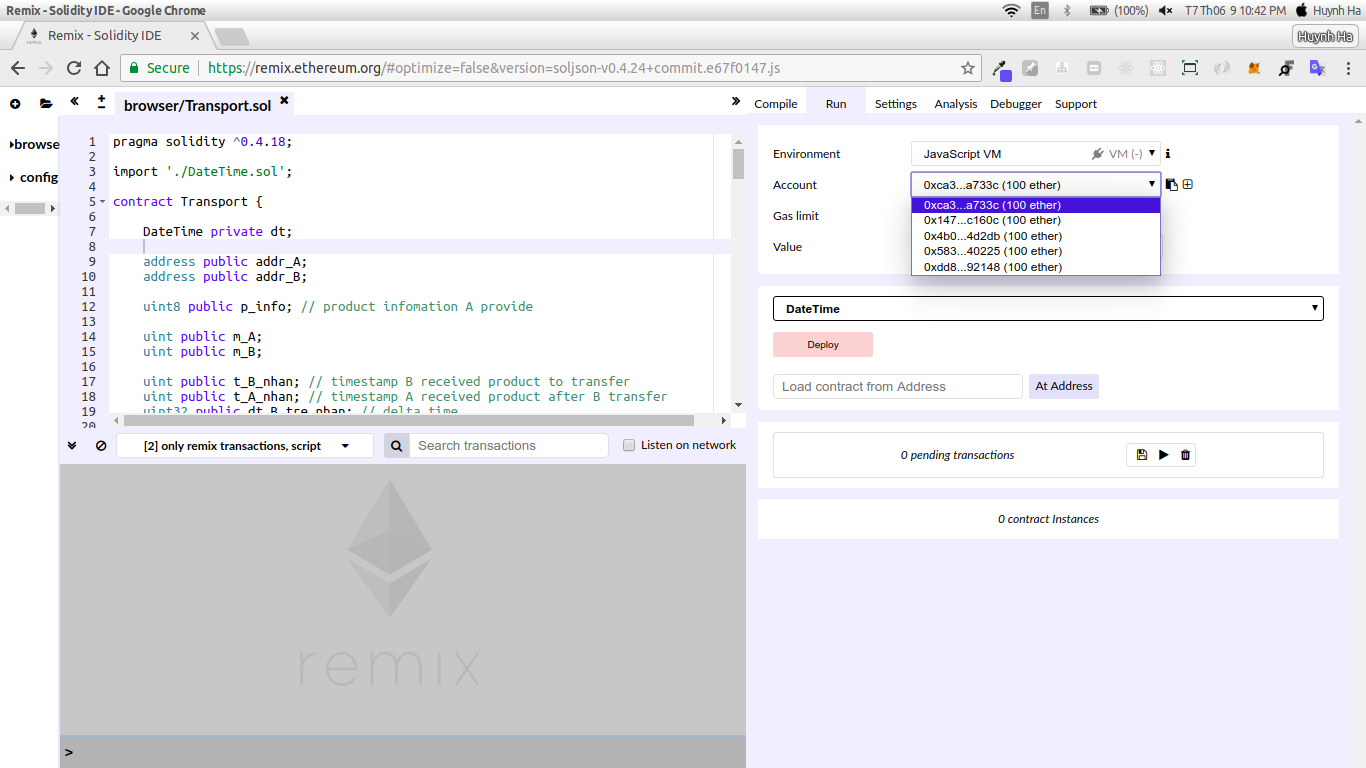
\includegraphics[width=14cm]{snapshot/2.png}
	\vspace{0.3cm}
	\caption{Compile smart contract}
	\label{fig:fig2}
\end{figure}

\begin{figure}[tph]
	\centering
	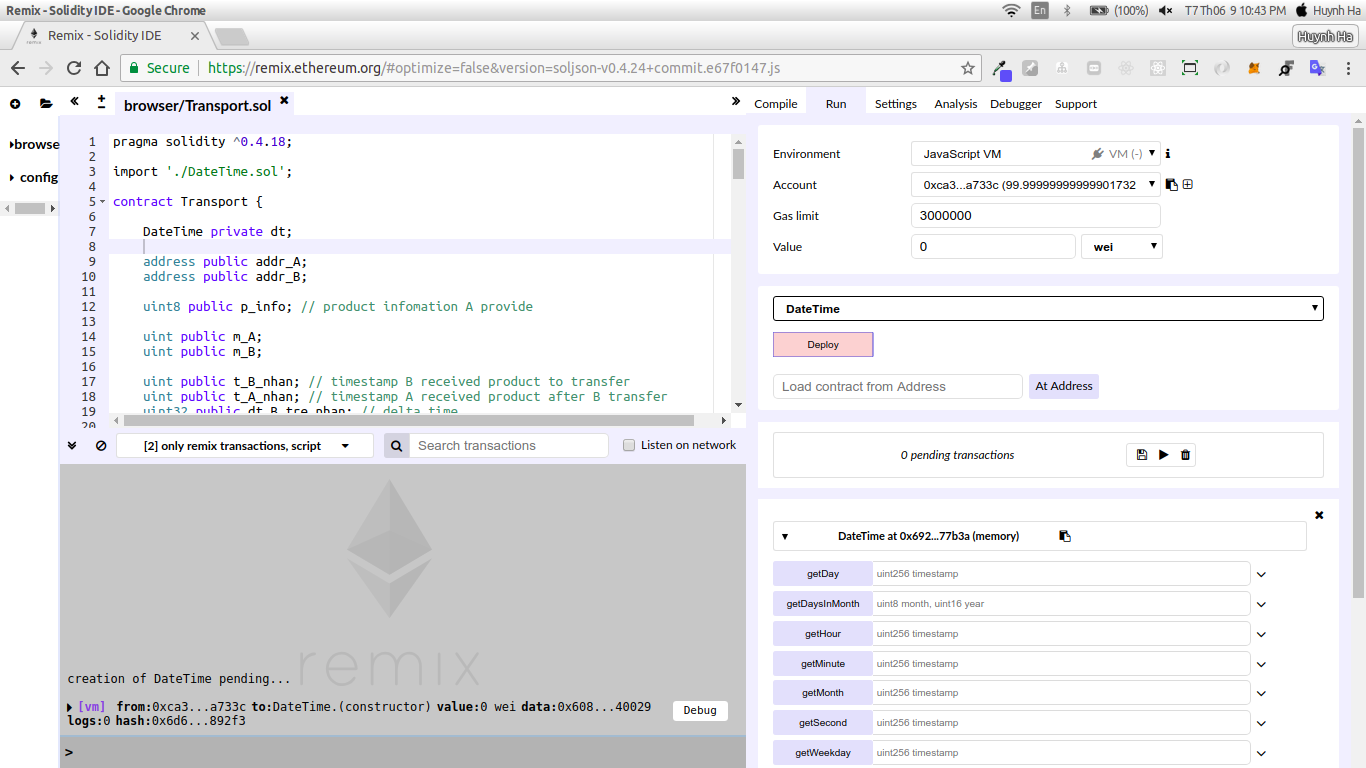
\includegraphics[width=14cm]{snapshot/3.png}
	\vspace{0.3cm}
	\caption{Môi trường chạy và các tài khoản tự sinh}
	\label{fig:fig3}
\end{figure}

\begin{figure}[tph]
	\centering
	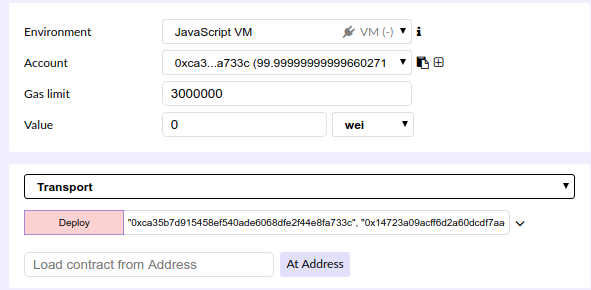
\includegraphics[width=14cm]{snapshot/4.png}
	\vspace{0.3cm}
	\caption{Deploy smart contract DateTime}
	\label{fig:fig4}
\end{figure}

\begin{figure}[tph]
	\centering
	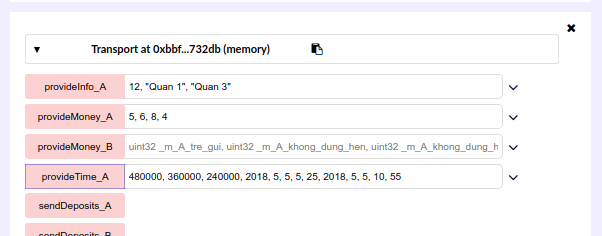
\includegraphics[width=14cm]{snapshot/5.png}
	\vspace{0.3cm}
	\caption{Deploy smart contract Transport}
	\label{fig:fig5}
\end{figure}

\begin{figure}[tph]
	\centering
	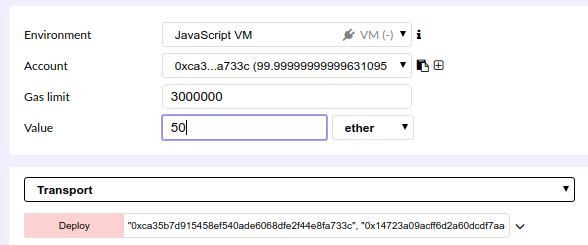
\includegraphics[width=14cm]{snapshot/6.png}
	\vspace{0.3cm}
	\caption{Thực thi các hàm bên A}
	\label{fig:fig6}
\end{figure}

\begin{figure}[tph]
	\centering
	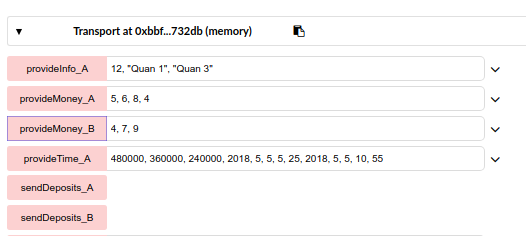
\includegraphics[width=14cm]{snapshot/7.png}
	\vspace{0.3cm}
	\caption{A gửi ether vào smart contract}
	\label{fig:fig7}
\end{figure}

\begin{figure}[tph]
	\centering
	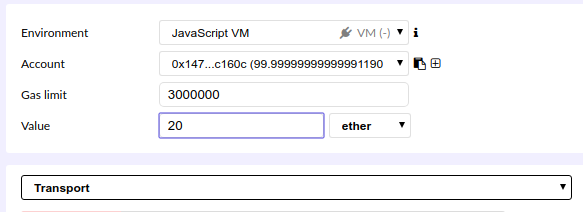
\includegraphics[width=14cm]{snapshot/8.png}
	\vspace{0.3cm}
	\caption{Thực thi các hàm bên B}
	\label{fig:fig8}
\end{figure}

\begin{figure}[tph]
	\centering
	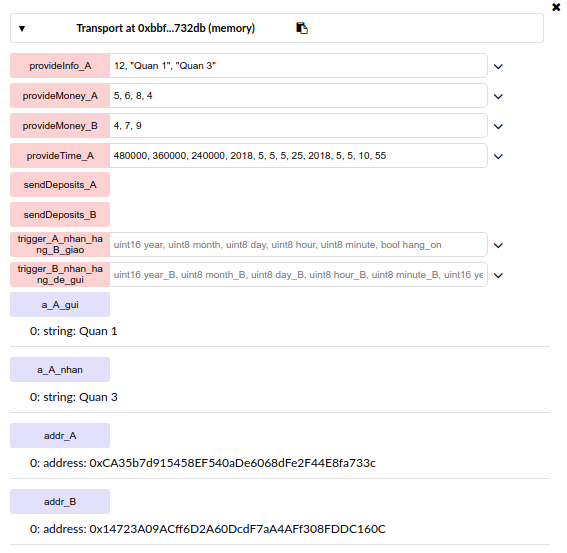
\includegraphics[width=14cm]{snapshot/9.png}
	\vspace{0.3cm}
	\caption{B gửi ether vào smart contract}
	\label{fig:fig9}
\end{figure}

\begin{figure}[tph]
	\centering
	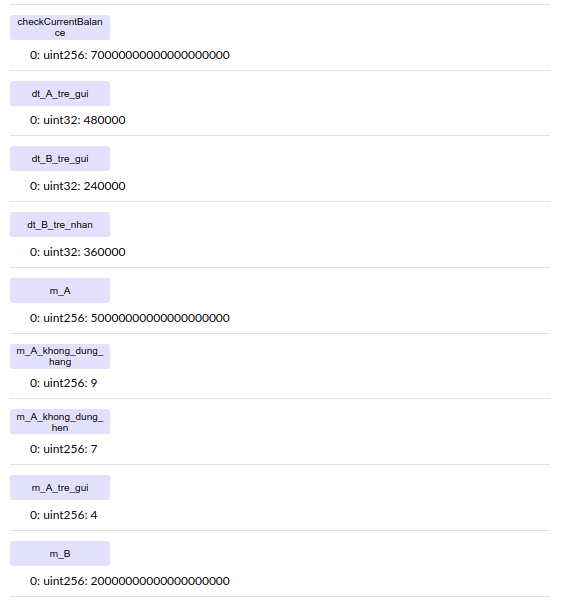
\includegraphics[width=14cm]{snapshot/10.png}
	\vspace{0.3cm}
	\caption{Các thông tin đầu vào smart contract (1)}
	\label{fig:fig10}
\end{figure}

\begin{figure}[tph]
	\centering
	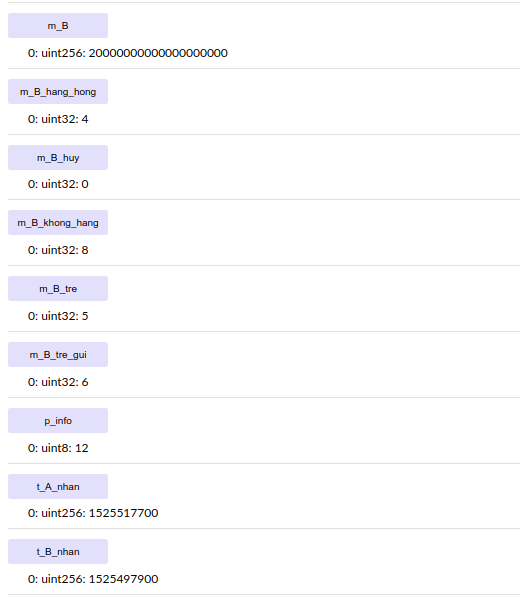
\includegraphics[width=14cm]{snapshot/11.png}
	\vspace{0.3cm}
	\caption{Các thông tin đầu vào smart contract (2)}
	\label{fig:fig11}
\end{figure}

\begin{figure}[tph]
	\centering
	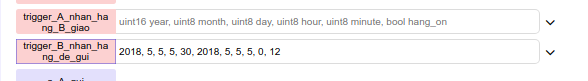
\includegraphics[width=14cm]{snapshot/12.png}
	\vspace{0.3cm}
	\caption{Các thông tin đầu vào smart contract (3)}
	\label{fig:fig12}
\end{figure}

\begin{figure}[tph]
	\centering
	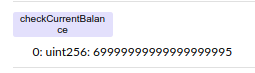
\includegraphics[width=8cm]{snapshot/13.png}
	\vspace{0.3cm}
	\caption{Thực thi khi B đến nhận hàng}
	\label{fig:fig13}
\end{figure}


\begin{figure}[tph]
	\centering
	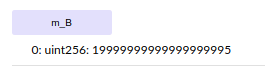
\includegraphics[width=8cm]{snapshot/14.png}
	\vspace{0.3cm}
	\caption{Kiểm tra tài khoản của B}
	\label{fig:fig14}
\end{figure}